% Vietnamese translation for OI Public Library
% Source-PDF: IOI中国国家候选队论文/2007/day2/10.刘家骅《浅谈随机化在信息学竞赛中的应用》.pdf
\documentclass[11pt]{article}
\usepackage{oipl-vn}
\usepackage{tikz}

\newcommand{\Oh}{\mathcal{O}}

\newcommand{\SawmillExampleFigure}{%
\begin{center}
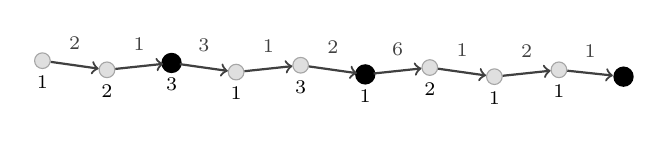
\begin{tikzpicture}[
  tree/.style={circle,draw=gray!70,fill=gray!25,inner sep=2pt},
  mill/.style={circle,fill=black,inner sep=2.6pt},
  edge/.style={->,black!75,thick},
  every node/.style={font=\scriptsize},
  x=0.82cm,y=0.58cm
]
  \foreach \i/\w/\yy in {0/1/0,1/2/-0.2,2/3/-0.05,3/1/-0.25,4/3/-0.1,5/1/-0.3,6/2/-0.15,7/1/-0.35,8/1/-0.2} {
    \node[tree] (t\i) at (\i,\yy) {};
    \node[below=2pt] at (t\i) {\w};
  }
  \node[mill] (m2) at (2,-0.05) {};
  \node[mill] (m5) at (5,-0.3) {};
  \node[mill] (end) at (9,-0.35) {};
  \foreach \a/\b/\d in {t0/t1/2,t1/t2/1,t2/t3/3,t3/t4/1,t4/t5/2,t5/t6/6,t6/t7/1,t7/t8/2,t8/end/1}
    \draw[edge] (\a)--node[above=2pt]{\d}(\b);
\end{tikzpicture}\\[-0.2em]
{\small Vị trí xưởng cưa tối ưu trong ví dụ Two Sawmills.}
\end{center}
}

\newcommand{\SearchMatrixFigure}{%
\begin{center}
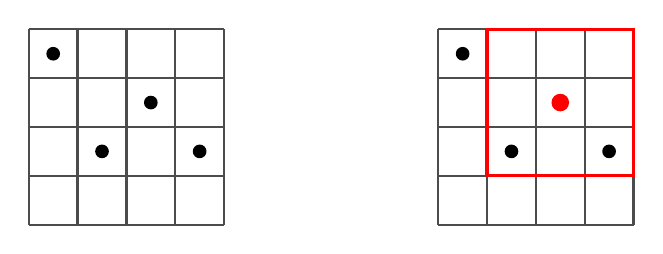
\begin{tikzpicture}[x=0.62cm,y=0.62cm]
  \draw[step=1,black!70,thick] (0,0) grid (4,4);
  \foreach \x/\y in {0.5/3.5,2.5/2.5,1.5/1.5,3.5/1.5}
    \fill[black] (\x,\y) circle (0.14);

  \begin{scope}[xshift=5.2cm]
    \draw[step=1,black!70,thick] (0,0) grid (4,4);
    \foreach \x/\y in {0.5/3.5,1.5/1.5,3.5/1.5}
      \fill[black] (\x,\y) circle (0.14);
    \fill[red] (2.5,2.5) circle (0.18);
    \draw[red,very thick] (1,1) rectangle (4,4);
  \end{scope}
\end{tikzpicture}\\[-0.2em]
{\small Chọn điểm ngẫu nhiên rồi thu hẹp ma trận tìm kiếm quanh điểm tốt nhất.}
\end{center}
}

\newcommand{\PartyGraphFigure}[1]{%
\begin{center}
\begin{tikzpicture}[
  v/.style={circle,draw,minimum size=0.55cm,inner sep=0pt,font=\small},
  light/.style={black!45,line width=0.6pt},
  heavy/.style={black,line width=1.8pt},
  every node/.style={font=\scriptsize}
]
  \node[v] (a) at (0,1.7) {1};
  \node[v] (b) at (3.1,2.0) {2};
  \node[v] (c) at (1.55,0.6) {3};
  \node[v] (d) at (0.55,-1.2) {4};
  \node[v] (e) at (3.8,-1.0) {5};
  \ifnum#1=1
    \draw[heavy] (a)--node[above]{5}(b);
    \draw[light] (a)--node[below left]{3}(c);
    \draw[heavy] (b)--node[right]{6}(c);
    \draw[light] (b)--node[right]{3}(e);
    \draw[heavy] (c)--node[left]{10}(d);
    \draw[heavy] (d)--node[above]{5}(e);
  \else
    \draw[light] (a)--node[above]{5}(b);
    \draw[heavy] (a)--node[below left]{3}(c);
    \draw[heavy] (b)--node[right]{6}(c);
    \draw[light] (b)--node[right]{3}(e);
    \draw[heavy] (c)--node[left]{10}(d);
    \draw[heavy] (d)--node[above]{5}(e);
  \fi
\end{tikzpicture}\\[-0.2em]
{\small \ifnum#1=1 Mạng liên lạc tối đa hóa tổng mức độ vui vẻ.%
\else Mạng liên lạc tối ưu sau khi thêm giới hạn bậc.\fi}
\end{center}
}

\title{Bàn sơ về ứng dụng ngẫu nhiên hóa trong thi tin học}
\author{Liu Jiahua}
\date{2007}

\begin{document}
\maketitle

\origtitle{A brief discussion of applications of randomization in informatics contests}
\sourcepath{IOI China candidate team papers / 2007 / day 2 / Liu Jiahua}

\section*{Tóm tắt}

Ngày nay, đề thi tin học thay đổi từng ngày, nhiều thuật toán mới liên tục
xuất hiện. Là một loại thuật toán tương đối mới, thuật toán ngẫu nhiên hóa
cũng đang phát huy vai trò độc đáo và quan trọng trên sân khấu thi tin học.

Bài viết này dùng một vài ví dụ điển hình để giới thiệu sơ lược ứng dụng của
thuật toán ngẫu nhiên hóa trong thi tin học.

\paragraph{Từ khóa.}
Thi tin học; ngẫu nhiên hóa.

\section*{Dẫn nhập}

Cùng với sự phát triển của thi tin học, cụm từ ``ngẫu nhiên hóa'' đã đi qua
một quá trình từ xa lạ đến quen thuộc trong suy nghĩ của học sinh dự thi.

Nhờ tính linh hoạt và biến hóa riêng của mình, thuật toán ngẫu nhiên hóa dần
dần được vận dụng khéo léo trong ngày càng nhiều kiểu đề khác nhau, và có ưu
thế riêng trong các cuộc thi tin học ngày càng đa dạng.

Nắm được thuật toán ngẫu nhiên hóa hiển nhiên giống như có thêm một công cụ
sắc bén để giải quyết bài toán.

\section{Một cách làm khác cho bài toán đơn giản}

\subsection*{Ví dụ: Geometrical dreams (Ural 1046)}

Cho một đa giác $A_1A_2\ldots A_N$. Trên mỗi cạnh $A_iA_{i+1}$, dựng về phía
ngoài đa giác một tam giác cân $A_iM_iA_{i+1}$ sao cho
$\angle A_iM_iA_{i+1}=\alpha_i$. Tập các góc $\alpha_i$ thỏa mãn điều kiện:
tổng góc của bất kỳ tập con không rỗng nào của nó đều không phải là bội của
$360^\circ$. Cho $N$, tọa độ của tất cả các điểm $M_i$ và các góc
$\alpha_i$; hãy viết chương trình xuất tọa độ các đỉnh của đa giác.

\subsection*{Phân tích}

Bài này có thể giải bằng cách lập và giải một hệ phương trình đơn giản.

Ta thử nhìn vấn đề từ một góc khác. Từ điều kiện của đề bài, dễ thấy rằng chỉ
cần xác định được tọa độ của một đỉnh, tọa độ các đỉnh còn lại của đa giác có
thể được tính ra bằng những phép tính đơn giản. Vì vậy bài toán được chuyển
thành việc xác định tọa độ của một đỉnh của đa giác.

Làm thế nào để xác định tọa độ của một đỉnh? Những thuật toán quen thuộc như
liệt kê hay chia đôi đều không giúp ta giải quyết trực tiếp, vì thế ta nghĩ
đến ngẫu nhiên hóa.

Ban đầu ta đặt điểm thứ nhất tại gốc tọa độ. Sau khi tính toán, ta thu được
tọa độ của đỉnh thứ $N+1$. Nếu đỉnh thứ $N+1$ trùng với đỉnh thứ nhất thì đa
giác này chính là đáp án cần tìm, nhưng xác suất xảy ra điều đó rõ ràng rất
nhỏ. Vì vậy ta phải điều chỉnh vị trí của điểm thứ nhất. Hiển nhiên khoảng
cách từ điểm thứ nhất đến điểm thứ $N+1$ càng nhỏ thì vị trí hiện tại càng
gần với vị trí thực sự của nó.

Mỗi lần, ta có thể chọn ngẫu nhiên một điểm ở gần vị trí tạm thời của điểm
thứ nhất, rồi xét xem nếu đặt điểm thứ nhất tại vị trí ấy thì khoảng cách
giữa điểm thứ nhất và điểm thứ $N+1$ có nhỏ hơn trước hay không. Nếu có, ta
tạm thời cố định điểm thứ nhất tại vị trí mới đó, rồi tiếp tục thao tác trên
cho đến khi điểm thứ nhất và điểm thứ $N+1$ trùng nhau. Khi đó ta xác định
được tọa độ các đỉnh của đa giác.

Thực tế chứng minh rằng phương pháp này có thể vượt qua bài toán. Dù cách
làm này hiển nhiên phức tạp hơn phương pháp thông thường đã nói ở trên về
mọi mặt, và không có nhiều ý nghĩa khi chỉ xét riêng bài này, nó đem lại cho
ta một hướng suy nghĩ hoàn toàn mới: ngẫu nhiên hóa.

Thuật toán ngẫu nhiên hóa không có ưu thế đối với bài kiểu này. Tuy nhiên nó
có thể được dùng trong rất nhiều vấn đề khác. Sau đây ta cùng xem thêm sức
hấp dẫn của thuật toán ngẫu nhiên hóa.

\section{Thử sức ban đầu}

\subsection*{Ví dụ: Two Sawmills (CEOI 2004)}

Trên con đường từ đỉnh núi xuống chân núi có $n$ cây cổ thụ. Chính quyền
quyết định chặt bỏ chúng; để không lãng phí gỗ, mỗi cây đều sẽ được vận
chuyển đến xưởng cưa.

Cây chỉ có thể được vận chuyển theo một hướng: xuống dốc. Ở cuối đường đã có
một xưởng cưa. Ngoài ra có thể xây thêm hai xưởng cưa tại vị trí của bất kỳ
cây nào trên đường. Bạn phải chọn nơi xây dựng sao cho chi phí vận chuyển là
nhỏ nhất. Chi phí vận chuyển là một xu cho mỗi mét và mỗi kilôgam gỗ.

Với dữ liệu ví dụ dưới đây, các cây được vẽ bằng vòng tròn có trọng lượng ghi
bên dưới, các xưởng cưa được tô đen, và cạnh trên đường đi ghi khoảng cách
giữa hai vị trí kề nhau.

\SawmillExampleFigure

\subsection*{Phân tích}

Thuật toán chuẩn cho bài này chuyển dữ liệu thành một hình ảnh hình học, rồi
dùng ngăn xếp để tính diện tích phủ lớn nhất của hai hình chữ nhật; độ phức
tạp thời gian là $\Oh(N)$. Tuy nhiên thuật toán này đòi hỏi năng lực không
nhỏ, và không dễ nghĩ ra.

Ta xem thuật toán ngẫu nhiên hóa biểu hiện thế nào trên bài này.

Cách ngẫu nhiên hóa dễ nghĩ nhất tất nhiên là chọn trực tiếp ngẫu nhiên hai
điểm, tính tổng chi phí vận chuyển khi lấy hai điểm đó làm xưởng cưa, lặp lại
nhiều lần rồi xuất giá trị nhỏ nhất.

Ta có thể tiền xử lý để hạ thời gian tính mỗi phương án xuống $\Oh(1)$. Khi
đó trong giới hạn thời gian ta có thể lấy ngẫu nhiên vài triệu, thậm chí vài
chục triệu lần. Nhưng so với tổng số trạng thái khoảng bốn trăm triệu, xác
suất tìm được nghiệm tối ưu vẫn không lớn.

Có phương pháp nào tốt hơn không?

Ở trên ta dùng thuật toán ngẫu nhiên hóa để trực tiếp sinh nghiệm, nên độ
chính xác không tốt. Để tăng độ chính xác, ta thử dùng ngẫu nhiên hóa để thu
hẹp phạm vi vùng tìm kiếm.

Ta dựng một ma trận $P$, trong đó $P[X,Y]$ biểu thị tổng chi phí vận chuyển
khi xưởng cưa thứ nhất được xây tại $X$ và xưởng cưa thứ hai được xây tại
$Y$. Ban đầu, cạnh của ma trận có độ dài $N$. Ta chọn ngẫu nhiên một số lượng
điểm nhất định trong ma trận. Số điểm được chọn nên tận dụng đầy đủ giới hạn
thời gian nhưng vẫn chú ý hiệu quả; vì kích thước ma trận liên tục thay đổi,
nên nên lấy số điểm theo một tỉ lệ cố định của kích thước ma trận. Sau đó ta
tính giá trị tại các điểm này, lấy điểm nhỏ nhất, dùng nó làm tâm của ma
trận mới, và lấy độ dài cạnh của ma trận mới bằng $3/4$ độ dài cạnh hiện tại.
Từ ma trận cũ, ta cắt ra một vùng làm phạm vi của ma trận mới; nếu phạm vi
ma trận mới vượt khỏi biên ma trận cũ thì dịch nó vào trong để nằm trọn trong
ma trận cũ. Tiếp tục lặp lại thao tác như vậy trên ma trận mới. Khi ma trận
mới đủ nhỏ, ta liệt kê mọi điểm trên ma trận ấy và lấy giá trị nhỏ nhất làm
đáp án.

Hình bên trái minh họa một ma trận tìm kiếm với vài điểm được chọn ngẫu nhiên.
Hình bên phải lấy điểm tốt nhất làm tâm, rồi cắt một ma trận con có cạnh bằng
$3/4$ cạnh hiện tại để tiếp tục tìm kiếm.

\SearchMatrixFigure

Thật đáng ngạc nhiên, thuật toán ngẫu nhiên hóa kiểu này có thể vượt qua toàn
bộ dữ liệu kiểm thử!

Qua bài toán này có thể thấy, tính linh hoạt và biến hóa của thuật toán ngẫu
nhiên hóa đem lại cho nó phạm vi ứng dụng rộng hơn. Ở nhiều chỗ tưởng như
khó bắt đầu, nếu vận dụng khéo léo thì nó có thể phát huy tác dụng. Chính
tính biến hóa ấy cũng đòi hỏi ta phải dùng thuật toán ngẫu nhiên hóa một cách
linh hoạt và thích đáng thì mới phát huy được ưu thế của nó. Thuật toán ngẫu
nhiên hóa không chỉ là tùy tiện làm bừa; khi dùng nó, cũng như với các thuật
toán khác, ta cần suy xét kỹ lưỡng và dụng công trong thiết kế.

Tiếp theo, ta xem phân tích cách dùng thuật toán ngẫu nhiên hóa trong một kỳ
thi thực tế.

\section{Phân tích thực chiến}

\subsection*{Ví dụ: Buổi tụ họp của Tiểu H (NOI 2005)}

Từ nhỏ Tiểu H đã rất thích máy tính; sau khi lên trung học, cậu càng say mê
lập trình. Sau nhiều năm cố gắng không ngừng, Tiểu H may mắn được chọn vào
đội tuyển thi tin học của tỉnh và sắp đến Trịnh Châu, Hà Nam, nơi cậu ngày
đêm mong nhớ, để dự kỳ thi Olympic Tin học Toàn quốc lần thứ 22 (NOI 2005).

Hai người bạn tốt của Tiểu H là Tiểu Y và Tiểu Z biết tin này, đều thật lòng
mừng cho cậu. Họ chuẩn bị tổ chức một buổi party, mời Tiểu H và tất cả bạn
bè của cậu tham dự để chúc mừng. Sau nhiều ngày điều tra, Tiểu Y và Tiểu Z
lập ra danh sách tất cả bạn tốt của Tiểu H; trong danh sách có tổng cộng $N$
người, để tiện ta đánh số họ từ $1$ đến $N$. Tuy nhiên danh sách quá dài, và
trong đó có không ít người mà Tiểu Y và Tiểu Z không quen. Làm thế nào để tổ
chức tất cả họ cùng tham gia buổi tụ họp?

Tiểu Y và Tiểu Z muốn thiết kế một mạng liên lạc cho $N$ người bạn của Tiểu
H, sao cho nếu một người biết tình hình mới nhất về buổi tụ họp thì những
người khác đều có thể nhận tin trực tiếp hoặc gián tiếp. Đồng thời, để bảo
đảm việc truyền tin đơn giản, hiệu quả, và quan trọng nhất là bí mật, vì họ
muốn tạo bất ngờ cho Tiểu H nên trong giai đoạn chuẩn bị tuyệt đối không thể
để cậu biết tin về buổi tụ họp, Tiểu Y và Tiểu Z quyết định để càng ít cặp
bạn liên lạc trực tiếp càng tốt. Muốn bảo đảm $N$ người bạn đều có thể liên
lạc trực tiếp hoặc gián tiếp với nhau, chỉ cần cho $(N-1)$ cặp bạn liên lạc
trực tiếp là đủ.

Rõ ràng những người trong danh sách không phải ai cũng quen nhau; ngay cả khi
hai người quen nhau, mức độ thân thiết giữa họ cũng khác nhau. Vì vậy Tiểu Y
và Tiểu Z lại dựa trên kết quả điều tra để lập bảng quan hệ giữa các bạn,
trong đó ghi rõ những người nào có thể liên lạc trực tiếp. Với mỗi cặp bạn có
thể liên lạc với nhau, họ còn ghi một mức độ vui vẻ khi liên lạc. Chẳng hạn,
quan hệ giữa $3$ và $4$ rất tốt, nên mức độ vui vẻ khi họ liên lạc được đánh
dấu là $10$; còn $1$ và $3$ chỉ là bạn bình thường, nên mức độ vui vẻ nhỏ hơn.

Hình 1 là một đồ thị với $N=5$: các đỉnh biểu thị bạn bè trong danh sách, các
cạnh biểu thị hai người có thể liên lạc trực tiếp, và số trên cạnh là mức độ
vui vẻ. Các cạnh được tô đậm tạo thành một mạng liên lạc có tổng mức độ vui vẻ
lớn nhất, bằng $5+6+10+5=26$.

\PartyGraphFigure{1}

Tiểu Y và Tiểu Z hy vọng mọi người đều thích buổi tụ họp này, nên quyết định
tối đa hóa mức độ vui vẻ của mạng liên lạc. Mức độ vui vẻ của một mạng liên
lạc được định nghĩa là tổng mức độ vui vẻ giữa mọi cặp người liên lạc trực
tiếp.

Tuy nhiên, nếu để một người trực tiếp liên lạc với rất nhiều người, điều đó
chắc chắn tạo gánh nặng lớn cho họ. Vì thế Tiểu Y và Tiểu Z còn đặt riêng
cho mỗi người một số lượng liên lạc trực tiếp tối đa $k_i$, nghĩa là trong
mạng liên lạc, nhiều nhất chỉ có $k_i$ người liên lạc trực tiếp với người
$i$. Vẫn dùng ví dụ ở Hình 1, nếu ta thêm các ràng buộc
$k_i=1,1,4,2,2$ cho các đỉnh từ $1$ đến $5$, thì phương án trên không còn
thỏa yêu cầu. Lúc này phương án tối ưu như Hình 2, với mức độ vui vẻ
$3+6+10+5=24$.

Hình 2 là đồ thị giống Hình 1 nhưng cây được chọn đổi thành các cạnh có trọng
số $3,6,10,5$, để thỏa các giới hạn bậc $1,1,4,2,2$.

\PartyGraphFigure{2}

Bạn có thể giúp Tiểu Y và Tiểu Z tìm một mạng liên lạc có mức độ vui vẻ càng
lớn càng tốt trong điều kiện thỏa các ràng buộc không?

\subsection*{Phân tích}

Đây là một bài nộp đáp án. Dữ liệu đề bài chia thành ba loại. Loại thứ nhất
gồm các dữ liệu $1$--$3$, trong đó giới hạn bậc của mỗi điểm đều là $N-1$,
tương đương không có giới hạn; có thể giải trực tiếp bằng thuật toán cây
khung nhỏ nhất. Loại thứ hai gồm các dữ liệu $4$--$6$, trong đó $N-1$ điểm có
giới hạn bậc là $N-1$, chỉ có một điểm có giới hạn bậc; có thể dùng thuật
toán cây khung nhỏ nhất có giới hạn bậc nhỏ nhất. Sách \textit{Nghệ thuật
thuật toán và thi tin học} có giới thiệu chi tiết.

Loại dữ liệu thứ ba gồm các dữ liệu $7$--$10$, trong đó mọi điểm đều có giới
hạn bậc; đây là một bài toán NP. Hơn nữa bài này là đề mở không yêu cầu nghiệm
tối ưu. Loại vấn đề như vậy chính là bầu trời rộng cho thuật toán ngẫu nhiên
hóa tự do phát huy.

Ta có thể dùng thuật toán ngẫu nhiên hóa kết hợp với các thuật toán khác nhau
để giải bài này.

\subsubsection*{Phương pháp 1: Thuật toán ngẫu nhiên hóa dựa trên Kruskal}

Ta dùng thuật toán Kruskal để tính một cây khung thỏa giới hạn bậc của các
điểm. Do có giới hạn bậc, cây khung thu được như vậy không nhất thiết là tối
ưu. Ta có thể sau khi sắp xếp cạnh theo trọng số, lại ngẫu nhiên xáo trộn thứ
tự một phần cạnh, rồi dùng thuật toán Kruskal để hy vọng thu được nghiệm tốt
hơn.

Mỗi lần thu được một cây khung tương đối lớn như vậy, ta lại ngẫu nhiên chọn
một cạnh không nằm trong cây khung, thêm nó vào cây khung để tạo thành một
chu trình, rồi trên chu trình ấy thử xóa một cạnh sao cho cây khung vẫn thỏa
giới hạn bậc và kết quả tốt hơn. Lặp lại nhiều lần như vậy, cho đến khi không
thể dùng cách này để thu được nghiệm tốt hơn nữa, tức đạt một nghiệm cực trị
cục bộ.

Sau khi chạy thuật toán Kruskal nhiều lần, ta xuất nghiệm tốt nhất tính được.

\subsubsection*{Phương pháp 2: Thuật toán ngẫu nhiên hóa dựa trên Prim}

Trước hết dùng thuật toán Prim để tính một cây khung lớn nhất khi chưa xét
giới hạn bậc.

Trên cây khung này, mỗi lần chọn ngẫu nhiên một điểm không thỏa giới hạn bậc,
rồi thử tìm một cạnh không nằm trong cây khung để thay cho một cạnh nằm trong
cây khung và nối với điểm đó, nhằm giảm bậc của điểm ấy. Dừng lại khi đã sửa
cây thành thỏa giới hạn bậc, hoặc khi không thể dùng cách này để giảm bậc của
các điểm vi phạm giới hạn.

Lặp lại thao tác trên nhiều lần từ cây khung lớn nhất ban đầu, rồi xuất nghiệm
tốt nhất tính được.

\subsubsection*{So sánh hai thuật toán}

\begin{center}
\begin{tabular}{c r r c r c}
\hline
 & & \multicolumn{2}{c}{Thuật toán 1} &
 \multicolumn{2}{c}{Thuật toán 2}\\
\cline{3-6}
Dữ liệu & Đáp án tham khảo & Kết quả ổn định\footnotemark & Điểm &
Kết quả ổn định & Điểm\\
\hline
7  & 64034   & 62712   & 7  & 63856   & 9\\
8  & 570138  & 565529  & 8  & 563403  & 8\\
9  & 1021302 & 1021385 & 10 & 1021461 & 10\\
10 & 1041394 & 1041604 & 10 & 1042087 & 10\\
\hline
\end{tabular}
\end{center}
\footnotetext{``Kết quả ổn định'' là kết quả nhận được trong đa số lần chạy
khi chạy chương trình nhiều lần.}

Qua ví dụ trên có thể thấy, dùng thuật toán ngẫu nhiên hóa trong đề mở có thể
thu được kết quả rất tốt. Việc kết hợp ngẫu nhiên hóa với các thuật toán khác
nhau sẽ cho kết quả khác nhau; khi giải bài, nên chọn thuật toán thích hợp để
phối hợp với ngẫu nhiên hóa nhằm nâng cao độ chính xác của chương trình.

\section*{Tổng kết}

Từ các bài toán trên có thể thấy, thuật toán ngẫu nhiên hóa có đặc điểm linh
hoạt và biến hóa. Khi áp dụng thuật toán ngẫu nhiên hóa, cần chú ý những điểm
sau:

\begin{itemize}
  \item Với các tình huống khác nhau, vận dụng thuật toán ngẫu nhiên hóa một
  cách linh hoạt, phát huy đầy đủ đặc điểm linh hoạt và biến hóa của nó.
  \item Chú ý kết hợp thuật toán ngẫu nhiên hóa với thuật toán thích hợp để
  kích phát sức mạnh lớn hơn.
  \item Chú ý hiệu quả của quyết định ngẫu nhiên và điều chỉnh ngẫu nhiên,
  tận dụng đầy đủ giới hạn thời gian mà đề bài cho.
\end{itemize}

Là một thuật toán mới nổi với đặc điểm rõ rệt, thuật toán ngẫu nhiên hóa không
chỉ cung cấp cho ta những cách khác nhau để giải rất nhiều bài toán, mà còn
có ưu thế rõ ràng trong các đề mở. Nắm vững và vận dụng linh hoạt thuật toán
ngẫu nhiên hóa chắc chắn sẽ giúp ta ứng biến tự nhiên hơn trên đấu trường tin
học luôn thay đổi.

\section*{Tài liệu tham khảo}

\begin{itemize}
  \item \textit{Nghệ thuật thuật toán và thi tin học}, Liu Rujia và Huang
  Liang.
  \item Slide buổi giảng đề NOI 2005.
\end{itemize}

\section*{Lời cảm ơn}

Cảm ơn các bạn Yang Yi, Kong Deben và Ye Shuxiong của Trường Trung học số 1
thành phố Shaoguan đã giúp đỡ.

Cảm ơn thầy Lin Shenghua đã bồi dưỡng và thầy Wei Jie đã ủng hộ.

Cảm ơn Bắc Cực Thiên Nam Tinh đã giúp đỡ với Ví dụ 1.

\appendix
\section{Phụ lục}

\subsection{Đề gốc: Geometrical dreams}

Có một đa giác $A_1A_2\ldots A_N$, các đỉnh $A_i$ được đánh số theo chiều kim
đồng hồ. Trên mỗi cạnh $A_iA_{i+1}$, dựng một tam giác cân
$A_iM_iA_{i+1}$ ở phía ngoài đa giác, và
$\angle A_iM_iA_{i+1}=\alpha_i$. Ở đây giả sử $A_{N+1}=A_1$.

Tập các góc $\alpha_i$ thỏa điều kiện rằng tổng các góc trong bất kỳ tập con
không rỗng nào của nó đều không chia hết cho $360^\circ$.

Cho $N$, tọa độ các đỉnh $M_i$ và các góc $\alpha_i$ đo theo độ. Hãy viết một
chương trình khôi phục tọa độ các đỉnh của đa giác.

\paragraph{Input.}
Dòng đầu chứa số nguyên $N$ ($3\le N\le 50$). $N$ dòng tiếp theo chứa các cặp
số thực $x_i,y_i$, là tọa độ của các điểm $M_i$
($-100\le x_i,y_i\le 100$). $N$ dòng cuối chứa giá trị theo độ của các góc
$\alpha_i$. Mọi số thực trong input có nhiều nhất $2$ chữ số sau dấu thập
phân.

\paragraph{Output.}
Output gồm $N$ dòng chứa tọa độ các điểm; dòng thứ $i$ chứa tọa độ của
$A_i$. Tọa độ phải chính xác đến $2$ chữ số sau dấu thập phân. Có thể giả sử
nghiệm luôn tồn tại.

\paragraph{Sample.}
\begin{verbatim}
input
3
0 2
3 3
2 0
90
90
90

output
1 1
1 3
3 1
\end{verbatim}

Tác giả bài: Dmitry Filimonenkov.

Nguồn bài: Ural State University collegiate programming contest
(25.03.2000).

\subsection{Two Sawmills}

Có $n$ cây cổ thụ được trồng dọc một con đường đi từ đỉnh đồi xuống chân đồi.
Chính quyền địa phương quyết định chặt chúng. Để không lãng phí gỗ, mỗi cây
phải được vận chuyển đến một xưởng cưa.

Cây chỉ có thể được vận chuyển theo một hướng: xuống dốc. Ở cuối đường phía
dưới đã có một xưởng cưa. Có thể xây thêm hai xưởng cưa dọc đường. Bạn phải
quyết định xây chúng ở đâu để tối thiểu hóa chi phí vận chuyển. Chi phí vận
chuyển là một xu cho mỗi mét, mỗi kilôgam gỗ.

\paragraph{Nhiệm vụ.}
Viết chương trình:
\begin{itemize}
  \item đọc từ input chuẩn số cây, trọng lượng và vị trí của chúng;
  \item tính chi phí vận chuyển nhỏ nhất;
  \item ghi kết quả ra output chuẩn.
\end{itemize}

\paragraph{Input.}
Dòng đầu chứa một số nguyên $n$, số cây ($2\le n\le 20000$). Các cây được
đánh số $1,2,\ldots,n$ bắt đầu từ đỉnh đồi và đi xuống. Mỗi dòng trong $n$
dòng tiếp theo chứa hai số nguyên dương cách nhau bằng một dấu cách. Dòng
$i+1$ chứa $w_i$, trọng lượng của cây thứ $i$ theo kilôgam, và $d_i$, khoảng
cách theo mét giữa cây thứ $i$ và cây thứ $i+1$; $1\le w_i\le 10000$,
$0\le d_i\le 10000$. Số cuối cùng trong các số này, $d_n$, là khoảng cách từ
cây thứ $n$ đến cuối đường phía dưới. Bảo đảm rằng tổng chi phí vận chuyển
tất cả cây đến xưởng cưa ở cuối đường nhỏ hơn $2\,000\,000\,000$ xu.

\paragraph{Output.}
Dòng đầu và duy nhất của output chứa một số nguyên: chi phí vận chuyển nhỏ
nhất.

\paragraph{Ví dụ.}
Với input:
\begin{verbatim}
9
1 2
2 1
3 3
1 1
3 2
1 6
2 1
1 2
1 1
\end{verbatim}

kết quả đúng là:
\begin{verbatim}
26
\end{verbatim}

Hình dưới minh họa vị trí tối ưu của các xưởng cưa trong ví dụ: cây được vẽ
bằng vòng tròn với trọng lượng ghi phía dưới; xưởng cưa được tô đen. Kết quả
bằng
\[
1\cdot(2+1)+2\cdot1+1\cdot(1+2)+3\cdot2+
2\cdot(1+2+1)+1\cdot(2+1)+1\cdot1=26.
\]

\SawmillExampleFigure

\subsection{Buổi tụ họp của Tiểu H}

\subsubsection*{Mô tả nhiệm vụ}

Từ nhỏ Tiểu H đã rất thích máy tính; sau khi lên trung học, cậu càng say mê
lập trình. Sau nhiều năm cố gắng không ngừng, Tiểu H may mắn được chọn vào
đội tuyển thi tin học của tỉnh và sắp đến Trịnh Châu, Hà Nam, nơi cậu ngày
đêm mong nhớ, để tham dự kỳ thi Olympic Tin học Toàn quốc lần thứ 22
(NOI 2005).

Hai người bạn tốt của Tiểu H là Tiểu Y và Tiểu Z biết tin này, đều thật lòng
mừng cho cậu. Họ chuẩn bị tổ chức một buổi party, mời Tiểu H và tất cả bạn
bè của cậu tham dự để chúc mừng. Sau nhiều ngày điều tra, Tiểu Y và Tiểu Z
lập ra danh sách tất cả bạn tốt của Tiểu H; trong danh sách có tổng cộng $N$
người, để tiện ta đánh số họ từ $1$ đến $N$. Tuy nhiên danh sách quá dài, và
trong đó có không ít người mà Tiểu Y và Tiểu Z không quen. Làm thế nào để tổ
chức tất cả họ cùng tham gia buổi tụ họp?

Tiểu Y và Tiểu Z muốn thiết kế một mạng liên lạc cho $N$ người bạn của Tiểu
H, sao cho nếu một người biết tình hình mới nhất về buổi tụ họp thì những
người khác đều có thể nhận tin trực tiếp hoặc gián tiếp. Đồng thời, để bảo
đảm việc truyền tin đơn giản, hiệu quả, và quan trọng nhất là bí mật, vì họ
muốn tạo bất ngờ cho Tiểu H nên trong giai đoạn chuẩn bị tuyệt đối không thể
để cậu biết tin về buổi tụ họp, Tiểu Y và Tiểu Z quyết định để càng ít cặp
bạn liên lạc trực tiếp càng tốt: để bảo đảm $N$ người bạn đều có thể liên
lạc trực tiếp hoặc gián tiếp với nhau, chỉ cần cho $(N-1)$ cặp bạn liên lạc
trực tiếp là đủ.

Rõ ràng những người trong danh sách không phải ai cũng quen nhau; ngay cả khi
hai người quen nhau, mức độ thân thiết giữa họ cũng khác nhau. Vì vậy Tiểu Y
và Tiểu Z lại dựa trên kết quả điều tra để lập bảng quan hệ giữa các bạn,
trong đó ghi rõ những người nào có thể liên lạc trực tiếp. Với mỗi cặp bạn có
thể liên lạc với nhau, họ còn ghi mức độ vui vẻ khi liên lạc.

Tiểu Y và Tiểu Z hy vọng mọi người đều thích buổi tụ họp này, nên quyết định
tối đa hóa mức độ vui vẻ của mạng liên lạc. Mức độ vui vẻ của một mạng liên
lạc là tổng mức độ vui vẻ giữa mọi cặp người liên lạc trực tiếp. Nếu để một
người trực tiếp liên lạc với rất nhiều người, điều đó sẽ tạo gánh nặng lớn
cho họ; vì vậy với mỗi người $i$ còn có giới hạn $k_i$, biểu thị trong mạng
liên lạc, nhiều nhất chỉ có $k_i$ người liên lạc trực tiếp với $i$.

Bạn có thể giúp Tiểu Y và Tiểu Z tìm một mạng liên lạc có mức độ vui vẻ càng
lớn càng tốt trong điều kiện thỏa các giới hạn không?

\paragraph{Định dạng input.}
Các file input \texttt{party1.in} đến \texttt{party10.in} đã được đặt trong
thư mục của người dùng.

Dòng đầu của mỗi file input gồm hai số nguyên $N$ và $M$. $N$ là tổng số bạn
của Tiểu H, $M$ là số cặp bạn tốt có thể liên lạc trực tiếp mà Tiểu Y và Tiểu
Z liệt kê được.

Dòng thứ hai chứa $N$ số nguyên trong phạm vi $[1,N-1]$, lần lượt mô tả
$k_1,k_2,\ldots,k_N$. Hai số kề nhau cách nhau bằng một dấu cách.

$M$ dòng tiếp theo, mỗi dòng mô tả một cặp bạn có thể liên lạc với nhau, theo
dạng \texttt{ui vi ci}. Điều này nghĩa là $u_i$ và $v_i$ có thể liên lạc trực
tiếp, và mức độ vui vẻ khi họ liên lạc là $c_i$.

Ngoài ra, ở cuối toàn bộ dữ liệu còn có một dòng riêng chứa một số thực $d$
trong phạm vi $(0,1]$ làm hệ số chấm điểm. Chương trình của bạn không cần
quan tâm đến tham số này, nhưng bạn có thể dựa vào gợi ý của tham số ấy để
thiết kế các thuật toán khác nhau. Mô tả về $d$ nằm trong phần chấm điểm bên
dưới.

\paragraph{Định dạng output.}
Đây là bài nộp đáp án. Bạn cần cung cấp mười file output từ
\texttt{party1.out} đến \texttt{party10.out}.

Dòng đầu của mỗi file là một số nguyên, biểu thị mức độ vui vẻ lớn nhất mà
bạn tìm được.

$(N-1)$ dòng tiếp theo mô tả mạng này. Mỗi dòng chứa một số $e_i$, biểu thị
trong mạng, cặp bạn được mô tả ở dòng thứ $(e_i+2)$ của file input sẽ liên
lạc trực tiếp.

\paragraph{Input mẫu.}
\begin{verbatim}
5 6
1 1 4 2 2
1 2 5
1 3 3
2 3 6
2 5 3
3 4 10
4 5 5
0.00001
\end{verbatim}

\paragraph{Output mẫu.}
\begin{verbatim}
24
2
3
5
6
\end{verbatim}

\paragraph{Giải thích mẫu.}
Xem ví dụ trong mô tả nhiệm vụ.

\paragraph{Cách chấm điểm.}
Bài này có điểm bộ phận. Với mỗi test:
\begin{itemize}
  \item Nếu phương án output không hợp lệ, chẳng hạn $e_i$ ngoài phạm vi,
  $e_i$ bị lặp, hoặc mạng không liên thông, test đó được $0$ điểm.
  \item Nếu phương án output không khớp với mức độ vui vẻ ghi ở dòng đầu của
  file output, test đó được $0$ điểm.
  \item Ngược lại, điểm của test được tính như sau. Đặt
  \[
    a=(1-d)\cdot\textit{our\_ans},\qquad
    b=(1+0.5d)\cdot\textit{our\_ans}.
  \]
  Nếu kết quả của bạn nhỏ hơn $a$, test đó được $0$ điểm. Nếu kết quả của bạn
  lớn hơn $b$, test đó được $15$ điểm. Nếu không, điểm của bạn là
  \[
    \textit{your\_score}
    =\left[
      \frac{\textit{your\_ans}-a}{\textit{our\_ans}}\cdot 10
    \right].
  \]
\end{itemize}
Trong đó $d$ là hệ số chấm điểm, tức số thực ở dòng cuối dữ liệu input;
\textit{our\_ans} là đáp án tham khảo do ban ra đề cung cấp, và
\textit{your\_ans} là đáp án của bạn.

\paragraph{Cách kiểm tra output của bạn.}
Ban tổ chức cung cấp công cụ \texttt{party\_check} để kiểm tra file output.
Cách dùng là nhập trên console:
\begin{verbatim}
./party_check <so thu tu test X>
\end{verbatim}

Sau khi gọi chương trình này, \texttt{party\_check} sẽ dựa trên file input
\texttt{partyX.in} và file output \texttt{partyX.out} của bạn để đưa ra kết
quả kiểm tra, gồm:
\begin{itemize}
  \item \texttt{Error: Not connected}: mạng liên lạc do chương trình xuất ra
  không liên thông.
  \item \texttt{Error: Edge xxx is duplicated}: cạnh thứ \texttt{xxx} được
  xuất hai lần.
  \item \texttt{Error: Edge in Line xxx is out of range}: cạnh mà chương trình
  xuất ở dòng thứ \texttt{xxx} không nằm trong phạm vi $[1,M]$.
  \item \texttt{Error: Degree of Friend xxx is out of range}: trong mạng liên
  lạc, số người liên lạc trực tiếp với bạn số \texttt{xxx} vượt quá giới hạn.
  \item \texttt{Error: Scheme \& happiness mismatch}: phương án và mức độ vui
  vẻ ở dòng đầu không khớp.
  \item Chương trình kiểm tra thoát bất thường: các trường hợp khác.
  \item \texttt{Correct! Happiness = xxx}: output đúng.
\end{itemize}

\paragraph{Chương trình nguồn.}
Bản gốc chỉ liệt kê tên các chương trình:
\begin{itemize}
  \item Ví dụ 1: \texttt{Geometrical dreams}, \texttt{timus1046.pas}.
  \item Ví dụ 2: \texttt{Two Sawmills}, \texttt{two.pas}.
  \item Ví dụ 3: \textit{Buổi tụ họp của Tiểu H}, phương pháp 1
  \texttt{party1.pas}, phương pháp 2 \texttt{party2.pas}.
\end{itemize}

\end{document}
